\section{Wall Times for Three Selected Tasks}
\label{app:select_time}

\begin{figure*}[!htb]
\centering
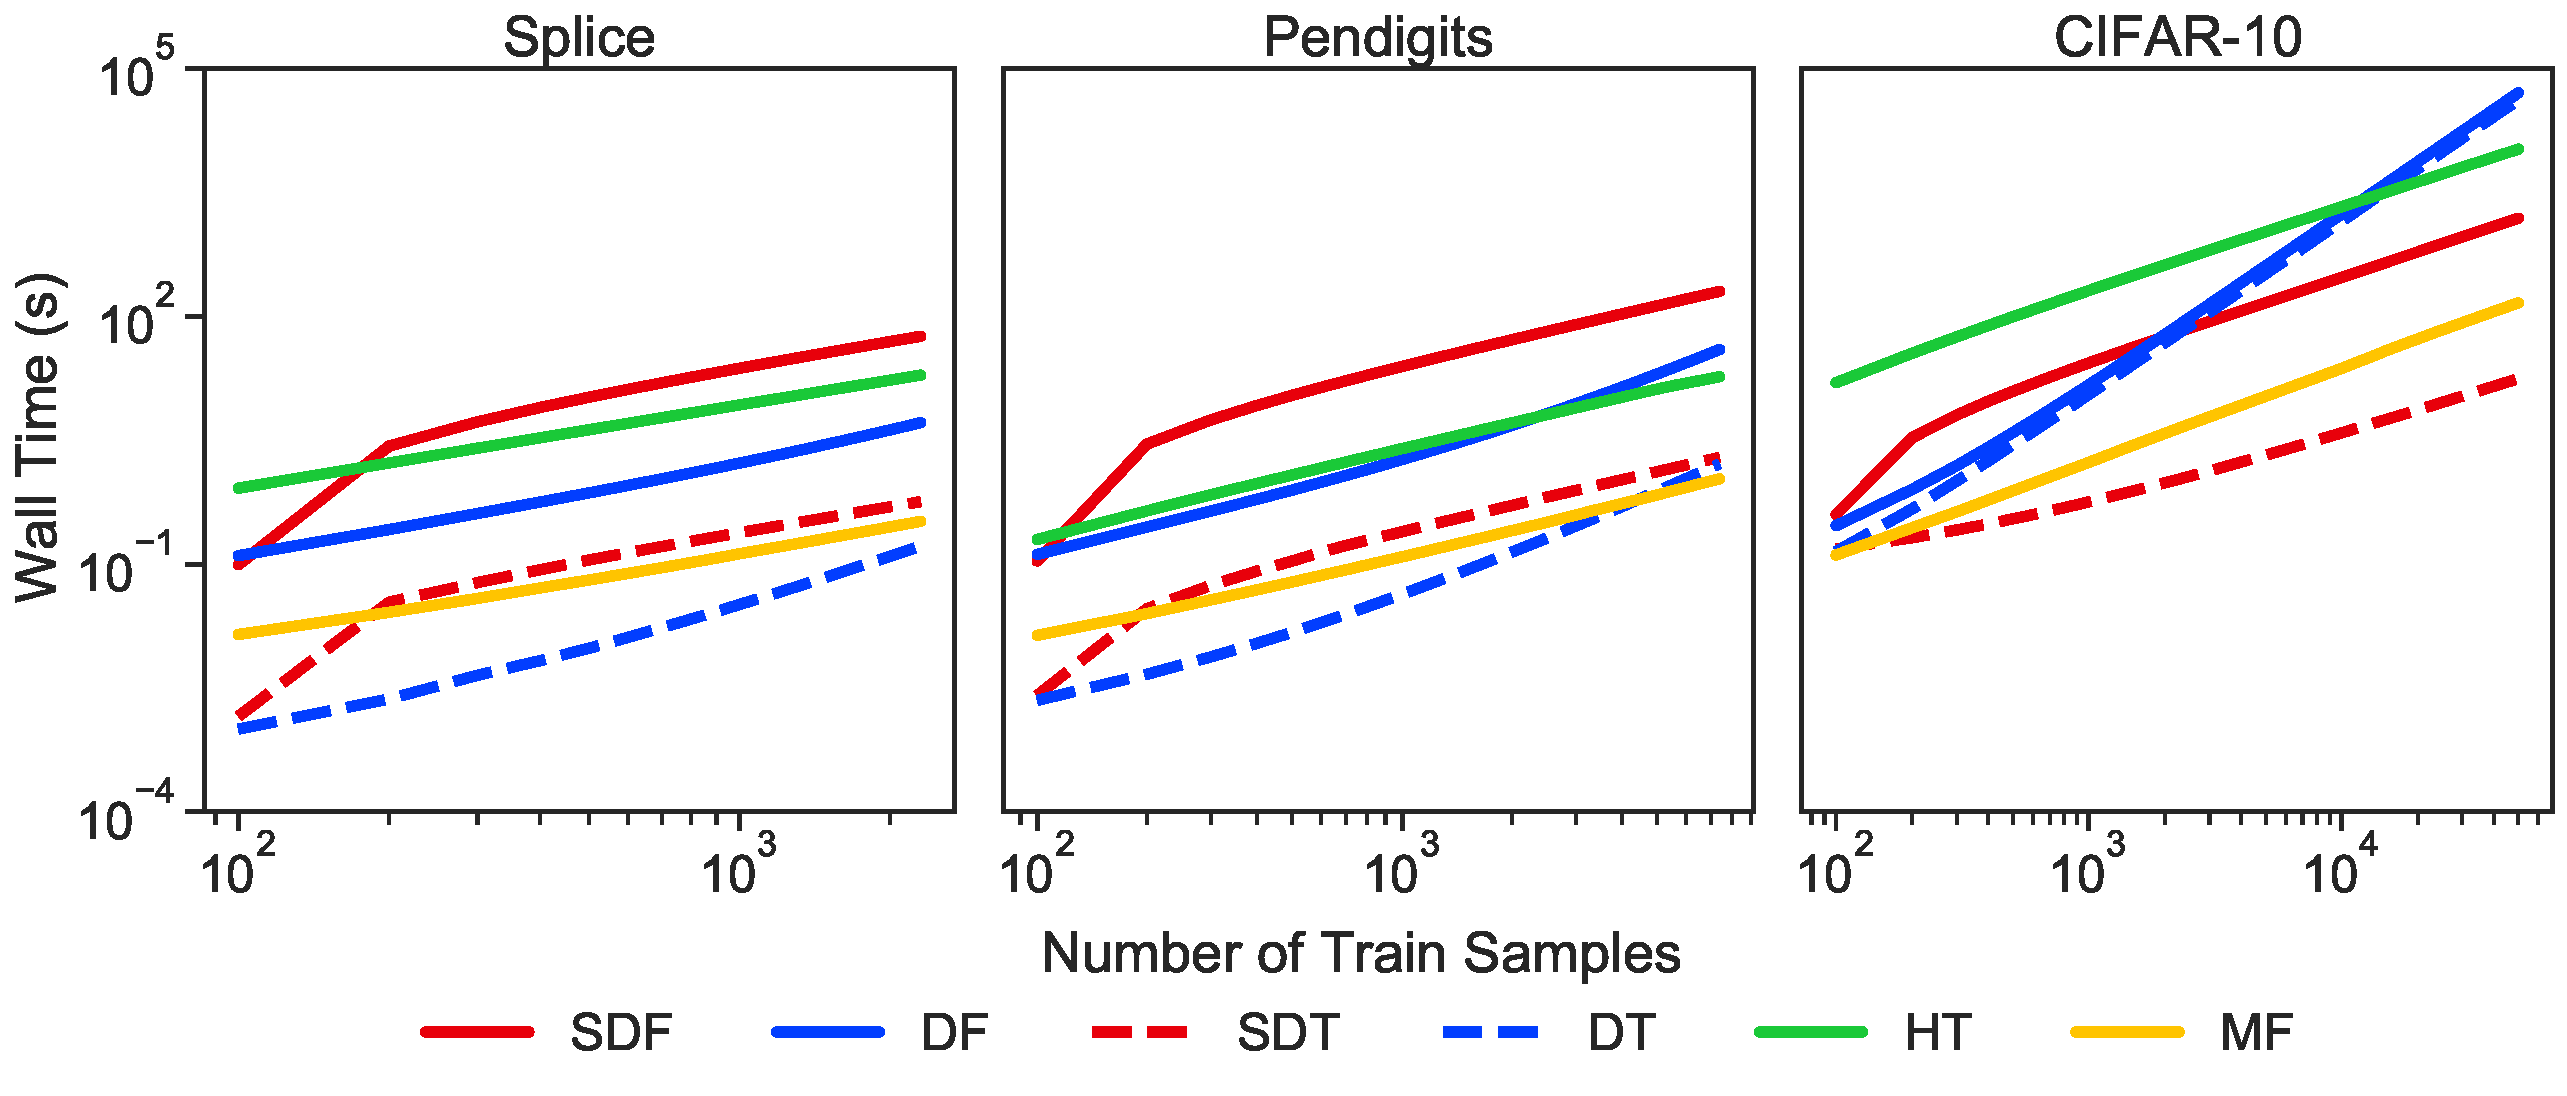
\includegraphics[width=0.9\textwidth]{select_time}
  \caption{Multiclass classifications on the Splice \textbf{(left)}, Pendigits \textbf{(center)}, and CIFAR-10 \textbf{(right)} datasets. The classifiers include: Stream Decision Forest \textbf{(SDF)}, Decision Forest \textbf{(DF)}, Stream Decision Tree \textbf{(SDT)}, Decision Tree \textbf{(DT)}, Hoeffding Tree \textbf{(HT)}, and Mondrian Forest \textbf{(MF)}. 
  Cumulative fitting times are shown for all estimators, and two batch estimators' times include refitting at each sample size. Each line represents averaged results from 10 random repetitions. SDTs are the most efficient in the CIFAR-10 task. SDFs take longer times in the Splice and Pendigits tasks, but the algorithm is overtaken by HTs, batch DTs, and DFs in the CIFAR-10 task. MFs with a limited amount of 10 trees are the most efficient forest classifier.
  }
\label{fig:select_time}
\end{figure*}

In terms of training wall times, SDTs are the most efficient on the CIFAR-10 dataset (Figure \ref{fig:select_time}, right). 
SDFs take longer times in the Splice and Pendigits tasks (Figure \ref{fig:select_time}, left and center). However, on the CIFAR-10 dataset, HTs are the most inefficient streaming trees, even slower than the two streaming ensembles. Also, as sample size increases, time usage of batch estimators grows more quickly due to refitting, and they surpass SDFs around 2,000 samples. MFs take shorter training times than other streaming forests, which could be attributed to a limited number of estimators (only 10 trees). All training wall times grow linearly as sample size increases.

\clearpage

\section{Accuracy for OpenML-CC18 Tasks}
\label{app:cc18}

\begin{figure}[!htpb]
\centering
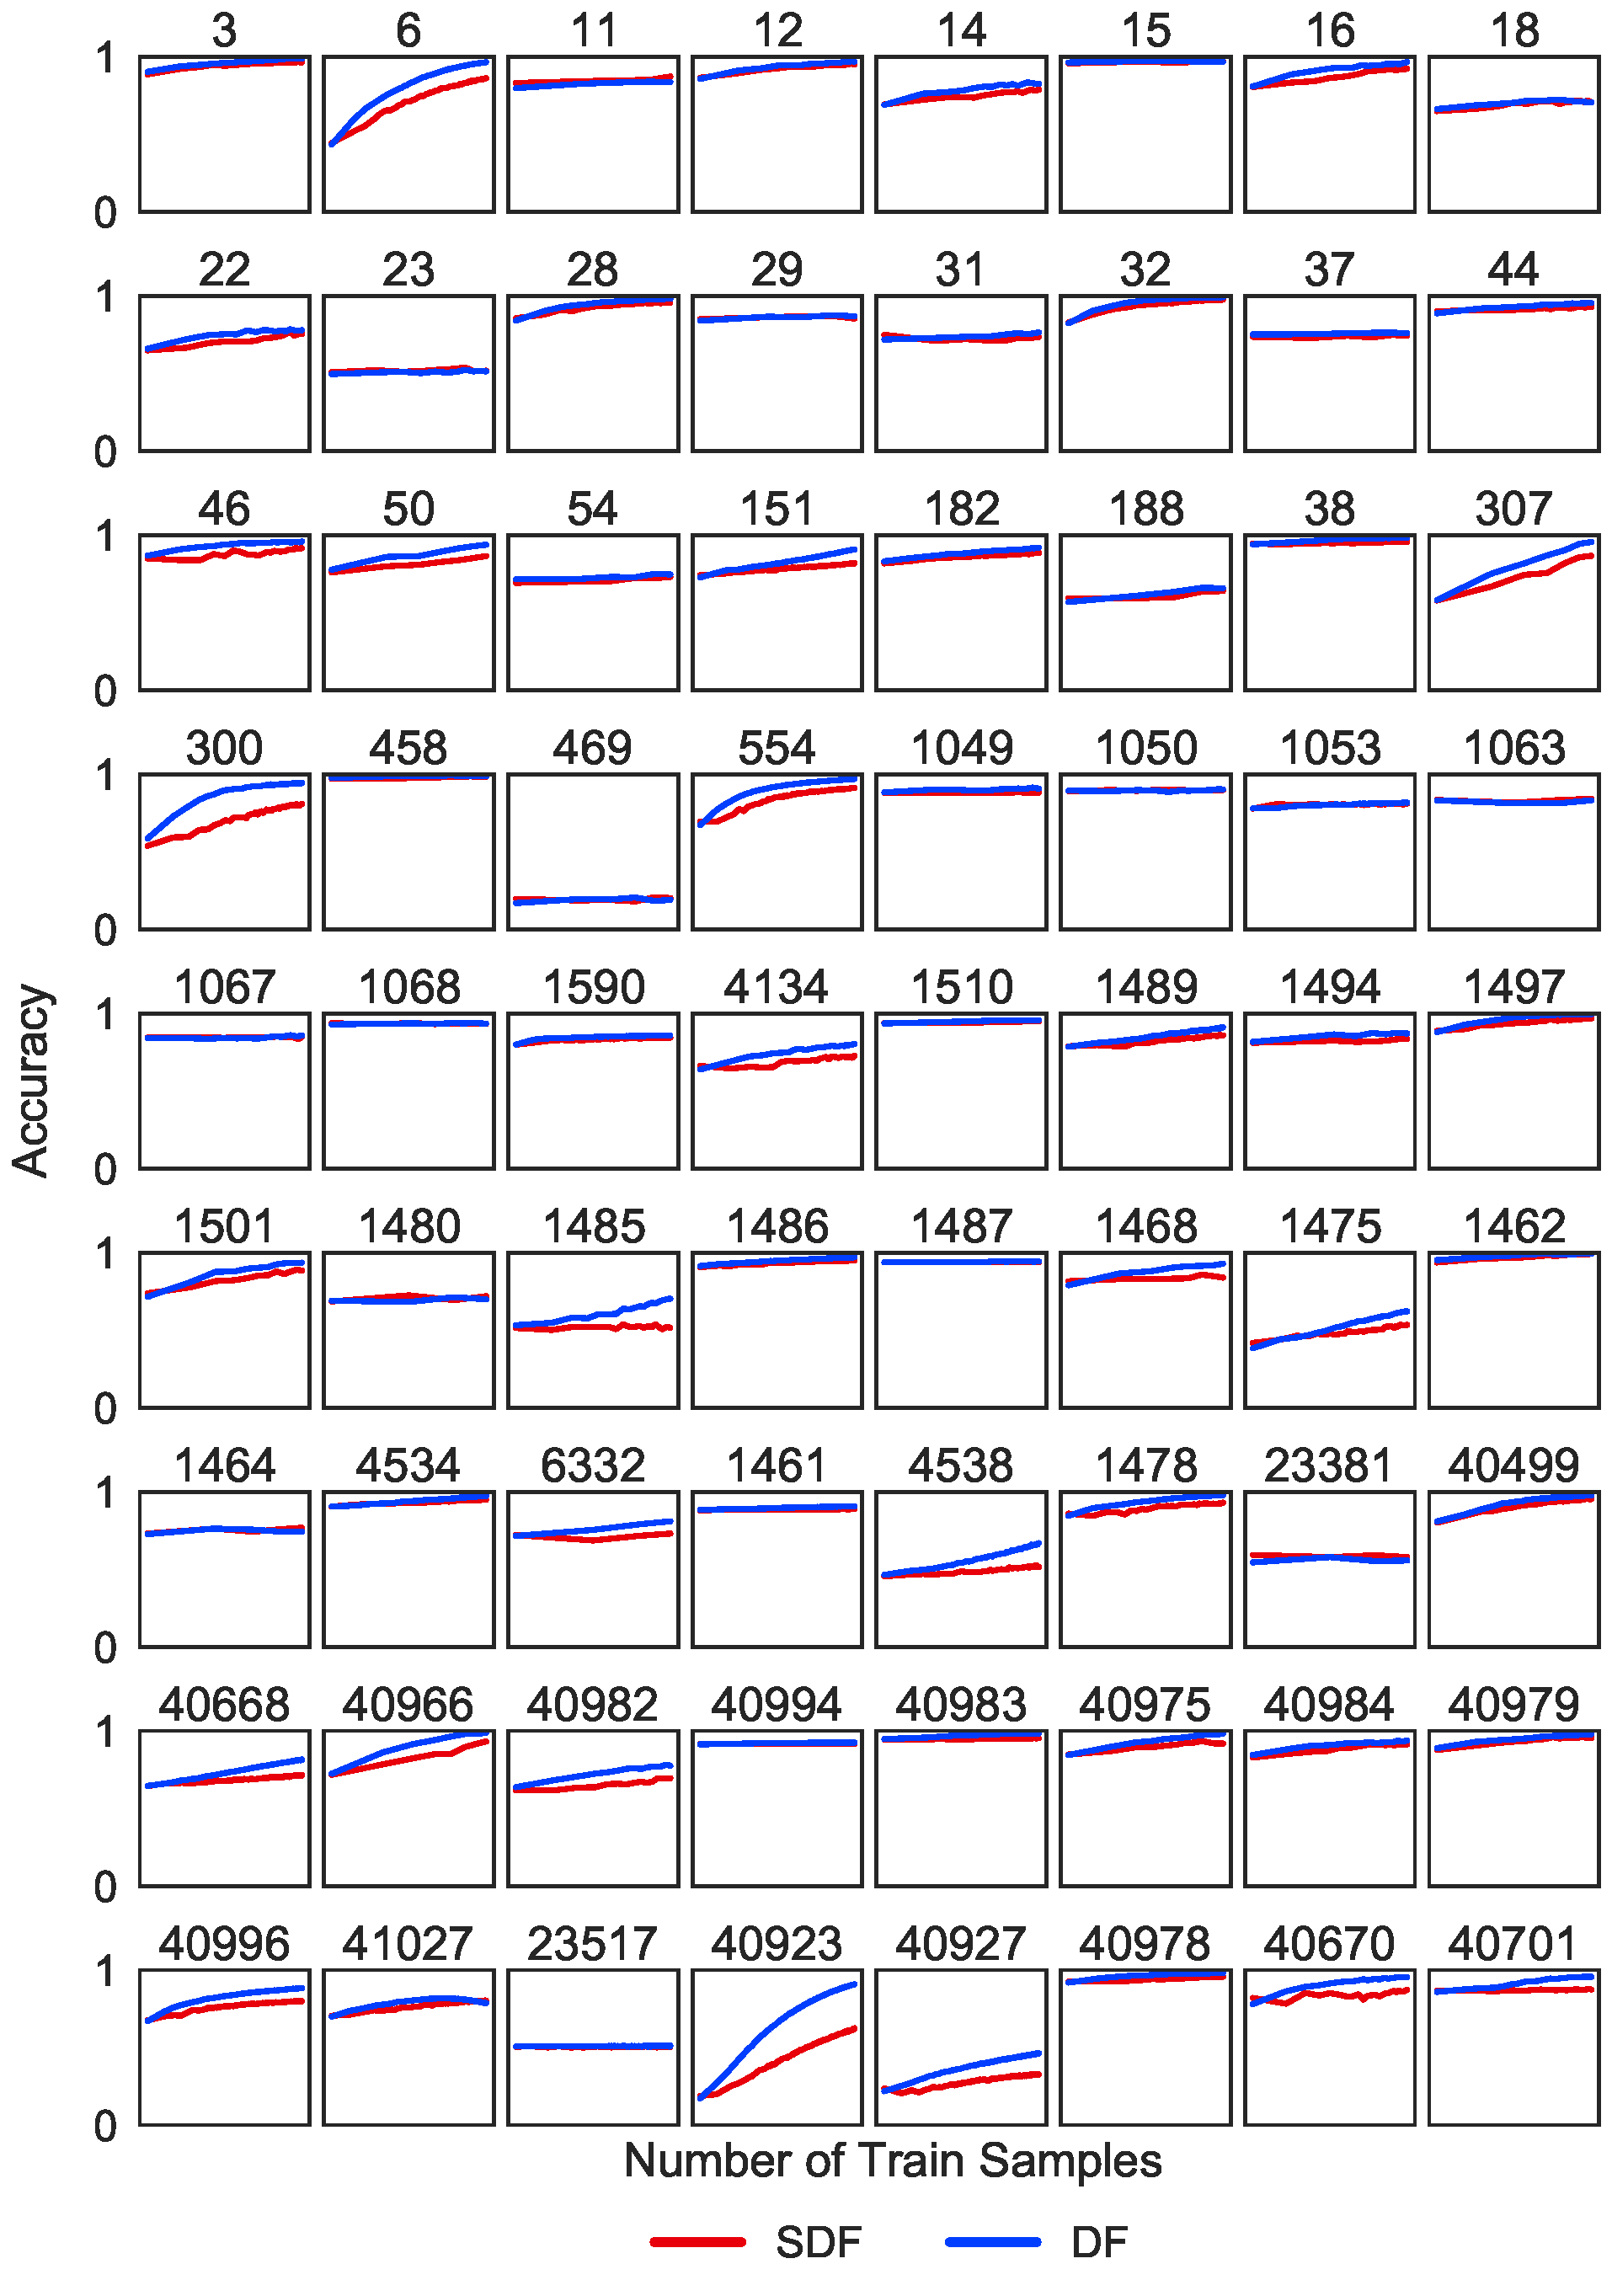
\includegraphics[width=0.75\columnwidth]{cc18_wide}
  \caption{Classifications on the OpenML-CC18 datasets with max sample size, number of features, and number of classes. The classifiers include: Stream Decision Forest \textbf{(SDF)} and Decision Forest \textbf{(DF)}. 
  All plots show averaged accuracy over five folds and are listed in the order of dataset IDs. Sample sizes correspond to respective datasets. In many tasks, SDFs perform as good, sometimes even better, than DFs. Moreover, SDF accuracy consistently increases with new samples across different data domains, which makes SDFs applicable to diverse real-world problems.
  }
\label{fig:cc18}
\end{figure}

